
\chapter{Reflectometry} \label{ch:Reflectometry}
\graphicspath{{chapter3_ys/}}
\minitoc


Reflectometry is a radar-like technique, which uses the reflection of waves inside the plasmas to measure the electron density and density fluctuations in fusion plasmas. Since the intensity of the waves is usually very low ($< 1$ W), the waves cause negligible perturbation to the local plasmas properties.

In this chapter, in section \ref{sec:EM_waves_propagation} we first provide the theoretical basis for reflectometry through propagation of electromagnetic waves in plasmas. The dispersion relations and the refraction index of EM waves in plasmas are derived from the Maxwell equations and plasma properties. This is followed by some important concepts, viz. polarization, resonance and cut-off. The effect of fluctuations on the wave propagation is discussed in section \ref{sec:effects_of_fluctuations}. Then, the experimental principles of reflectometry are presented in section \ref{sec:reflectometry_principles}. Finally, in section \ref{sec:drefluc} we focus on the core reflectometry diagnostic at Tore Supra, as well as the density fluctuation measurements by this diagnostic that are used in this study.


\section{Electromagnetic waves propagation in plasmas} \label{sec:EM_waves_propagation}

Wave propagation in magnetized plasmas is significantly more complicated compared to propagation in non-magnetized media, as the magnetic field causes highly anisotropic dynamics parallel and perpendicular to the magnetic field. We therefore focus first on the basics of EM wave propagation in magnetized plasmas, before proceeding to the particularities of wave propagation for reflectometry applications.


\subsection{Dispersion relation} \label{sec:dispersion_relation}

In the MHD approach to plasma dynamics, a plasma is treated as a continuous medium wherein currents can flow. The corresponding electric and magnetic fields have to obey the Maxwell equations, the differential forms of which are:%
%%%%%%%%%%%%%%%%%%%%
\begin{equation}\label{eq:maxwellE}
    \nabla \times \bu{E} = -\dxdt{\bu{B}}{t},
\end{equation}
%%%%%%%%%%%%%%%%%%%%
%%%%%%%%%%%%%%%%%%%%
\begin{equation}\label{eq:maxwellB}
    \nabla \times \bu{B} = \mu_0\bu{j} + \frac{1}{c^2}\dxdt{\bu{E}}{t}.
\end{equation}
%%%%%%%%%%%%%%%%%%%%
\noindent The plasma properties are reflected by the current density $\bu{j}$. There could be unperturbed (or equilibrium) values of the magnetic and electric fields $\bu{B_0}$ and $\bu{E_0}$ that are independent of the waves being considered. In this case, \eqref{eq:maxwellE} and \eqref{eq:maxwellB} are applied to the unperturbed and wave parts separately and here only the wave parts are considered. One can eliminate $\bu{B}$ by taking $\nabla \times$ of \eqref{eq:maxwellE} and $\frac{\partial}{\partial{t}}$ of the second, amounting to the following wave equation:%
%%%%%%%%%%%%%%%%%%%%
\begin{equation}\label{eq:wave}
    \nabla \times (\nabla \times \bu{E}) + \frac{\partial}{\partial{t}}\left( \mu_0\bu{j} + \frac{1}{c^2}\dxdt{\bu{E}}{t} \right) = 0.
\end{equation}
%%%%%%%%%%%%%%%%%%%%

Now, assuming that the wave fields are small compared to the equilibrium values and that the plasma is spatially homogeneous, the wave fields can be expressed by the sum of Fourier series (modes):%
%%%%%%%%%%%%%%%%%%%%
\begin{equation}\label{eq:fourier_transform}
  \bu{E}(\bu{x},t)=\int \bu{E}(\bu{k},\omega)e^{i(\bu{k}\cdot\bu{x}-\omega{t})}\mathrm{d}\bu{k}\mathrm{d}\omega,
\end{equation}
%%%%%%%%%%%%%%%%%%%%
\noindent where each Fourier mode $\bu{E}(\bu{k},\omega)$ satisfies \eqref{eq:wave}. As the wave fields are small, the current ($\bu{j}$) is a linear function of the electric field ($\bu{E}$). Therefore, for each Fourier mode, the relation between $\bu{j}$ and \bu{E} can be expressed by Ohm's law:%
%%%%%%%%%%%%%%%%%%%%
\begin{equation}\label{eq:ohm_law}
  \bu{j}(\bu{k},\omega)=\bu{\sigma}(\bu{k},\omega) \cdot \bu{E}(\bu{k},\omega),
\end{equation}
%%%%%%%%%%%%%%%%%%%%
\noindent where $\bu{\sigma}$ is the conductivity of the plasma. In general for an anisotropic plasma, $\bu{\sigma}$ becomes the conductivity tensor, which will be discussed later.

Next, through the Fourier transform $\bu{E}(\bu{x},t) \rightarrow \bu{E}(\bu{k},\omega)$ ($\frac{\partial}{\partial{t}} \rightarrow -i\omega, \nabla \rightarrow ik\bu{e_x}$) and linearization, \eqref{eq:wave} becomes:%
%%%%%%%%%%%%%%%%%%%%
\begin{equation}\label{eq:matrix}
   \left( \bu{k}\bu{k} - k^2\bu{I} + \frac{\omega^2}{c^2}\boldsymbol{\epsilon} \right) \cdot \bu{E} = 0,
\end{equation}
%%%%%%%%%%%%%%%%%%%%
\noindent where $\bu{I}$ is the second-order unit tensor and $\bu{\epsilon}$ the dielectric tensor of the plasma:%
%%%%%%%%%%%%%%%%%%%%
\begin{equation}\label{eq:dielectric_definition}
  \bu{\epsilon} = \bu{I} + \frac{i}{\omega\varepsilon_0}\bu{\sigma}.
\end{equation}
%%%%%%%%%%%%%%%%%%%%
\noindent The dielectric tensor is a more convenient quantity to describe the properties of the plasma than the conductivity.

Now \eqref{eq:matrix} represents three homogeneous simultaneous equations for the three components of the electric fields $\bu{E}$. To have a nontrivial (nonzero) solution, the determinant of the matrix coefficients must be zero:%
%%%%%%%%%%%%%%%%%%%%
\begin{equation}\label{eq:det_dispersion_relation}
   \mathrm{det}\left( \bu{k}\bu{k} - k^2\bu{I} + \frac{\omega^2}{c^2}\boldsymbol{\epsilon} \right)=0.
\end{equation}
%%%%%%%%%%%%%%%%%%%%
\noindent This equation determines relations between the wavenumber $\bu{k}$ and the frequency $\omega$ for the different waves. The solutions $k=f(\omega)$, called the eigenvalues of the matrix equation, provide the \emph{dispersion relation} of these waves. The solutions for $\bu{E}$, called the eigenvector, determines the polarization characteristics of these waves.


\subsection{Refractive index} \label{sec:refractive_index}

From the previous derivation we know that the particular properties of plasmas affect the wave propagation through the conductivity $\bu{\sigma}$ or the permittivity $\bu{\epsilon}$. To calculate the plasma permittivity, the kinetic treatment by the Boltzmann equation considers the distribution function of particles in phase-space and thus provides a comprehensive plasma information. Here, we use the fluid treatment which considers only the zeroth moment of the Boltzmann equation, i.e. the density. The simplified fluid approach is adequate in our case when the waves travel at phase velocities close to the speed of light in plasmas whose electron thermal velocity is much less than the speed of light ($\upsilon_{th} \ll c$). When neglecting the particle thermal motion, the treatment is called the \emph{cold plasma} approximation.

The equation of motion of a single electron in a plasma is:%
%%%%%%%%%%%%%%%%%%%%
\begin{equation}\label{eq:eletron_motion}
   m_e\dxdt{\bu{v}}{t} = -e(\bu{E}+\bu{v}\times\bu{B_0}),
\end{equation}
%%%%%%%%%%%%%%%%%%%%
\noindent here, an unperturbed magnetic field $\bu{B_0}$ is considered but collisions are ignored. In the cold plasma approximation the electrons move together and the current density becomes:%
%%%%%%%%%%%%%%%%%%%%
\begin{equation}\label{eq:current_density}
  \bu{j}=-en_e\bu{v}=\bu{\sigma} \cdot \bu{E}.
\end{equation}
%%%%%%%%%%%%%%%%%%%%
\noindent For simplicity and without loss of generality, taking $\bu{B_0}$ in the direction of the $z$ axis, the conductivity tensor is obtained from the three components of \eqref{eq:eletron_motion} and \eqref{eq:current_density}:%
%%%%%%%%%%%%%%%%%%%%
\begin{equation}\label{eq:conductivity_tensor}
  \bu{\sigma} = \frac{in_ee^2}{m_e\omega} \cdot \frac{1}{1-\omega_{ce}^2/\omega^2}
\begin{bmatrix}
\vspace{0.5cm}
1 & -i\omega_{ce}/\omega & 0 \\
\vspace{0.5cm}
\omega_{ce}/\omega & 1 & 0 \\
0 & 0 & 1-\omega_{ce}^2/\omega^2
\end{bmatrix}.
\end{equation}
%%%%%%%%%%%%%%%%%%%%
\noindent Here, $e$, $n_e$ and $m_e$ are the electron charge, density and mass, respectively, while $\omega_{ce}=eB_0/m_e$ is the electron cyclotron frequency. This is only the electron conductivity, whereas the total conductivity has contributions from both electrons and ions. The same derivation and results are valid for the ions, except that one should use the ion charge, density and mass ($Ze$, $n_i$, $m_i$) in \eqref{eq:conductivity_tensor}. Because $m_i \ll m_e$, the ion conductivity is negligible when compared to the electron contribution, as long as the wave frequency is sufficiently high. According to the definition \eqref{eq:dielectric_definition}, the dielectric tensor can be written as:%
%%%%%%%%%%%%%%%%%%%%
\begin{equation}\label{eq:dielectric_tensor}
\bu{\epsilon} =
\begin{bmatrix}
\vspace{0.5cm}
1-\frac{\omega_{pe}^2}{\omega^2-\omega_{ce}^2} & \frac{i\omega_{pe}^2\omega_{ce}}{\omega(\omega^2-\omega_{ce}^2)} & 0 \\
\vspace{0.5cm}
\frac{-i\omega_{pe}^2\omega_{ce}}{\omega(\omega^2-\omega_{ce}^2)} & 1-\frac{\omega_{pe}^2}{\omega^2-\omega_{ce}^2} & 0 \\
0 & 0 & 1-\frac{\omega_{pe}^2}{\omega^2}
\end{bmatrix},
\end{equation}
%%%%%%%%%%%%%%%%%%%%
\noindent where $\omega_{pe}=(n_ee^2/\varepsilon_0m_e)^{1/2}$ is the electron plasma frequency.

For convenience, the following dimensionless physical quantities are defined:%
%%%%%%%%%%%%%%%%%%%%
\begin{equation}
   X = \frac{\omega_{pe}^2}{\omega},  Y = \frac{\omega_{ce}}{\omega},  N = \frac{kc}{\omega}.
\end{equation}
%%%%%%%%%%%%%%%%%%%%
\noindent Then, substituting $\bu{\epsilon}$ from \eqref{eq:dielectric_tensor} into \eqref{eq:det_dispersion_relation}, the determinant equation becomes:%
%%%%%%%%%%%%%%%%%%%%
\begin{equation}
\begin{vmatrix}
\vspace{0.5cm}
-N^2+1-\frac{X}{1-Y^2} & \frac{iXY}{1-Y^2} & 0 \\
\vspace{0.5cm}
-\frac{iXY}{1-Y^2} & -N^2\cos^2\theta+1-\frac{X}{1-Y^2} & N^2\cos\theta\sin\theta \\
0 & N^2\cos\theta\sin\theta & -N^2\sin^2\theta+1-X
\end{vmatrix} = 0.
\end{equation}
%%%%%%%%%%%%%%%%%%%%
\noindent Here, $\theta$ is the angle between the wavenumber $\bu{k}$ and the magnetic field $\bu{B_0}$. The solutions are of the following form:%
%%%%%%%%%%%%%%%%%%%%
\begin{equation}
N^2 = 1 - \frac{X(1-X)}{1-X-\frac{1}{2}Y^2\sin^2\theta\pm[(\frac{1}{2}Y^2\sin^2\theta)^2+(1-X)^2Y^2\cos^2\theta]^{1/2}}.
\end{equation}
%%%%%%%%%%%%%%%%%%%%
\noindent This is called the \emph{Appleton-Hartree formula} for the refractive index $N$. Two main situations exist, depending on the angle between $\bu{k}$ and $\bu{B_0}$:
%
\begin{itemize}
  \item $\bu{k} \parallel \bu{B_0}$ ($\theta = 0$): the waves propagate parallel to the magnetic field and the solutions are %
      %%
      \begin{equation}
        N^2=1-\frac{X}{1-Y^2}\pm\frac{XY}{1-Y^2}.
      \end{equation}
      %%
      Here, the waves are circularly polarized and '+' and '-' correspond to left- and right-handed electric field rotation, respectively.
%
  \item $\bu{k} \perp \bu{B_0}$ ($\theta = \pi/2$): the waves propagate perpendicular to the magnetic field with solutions %
      %%
      \begin{equation}\label{eq:Omode_index}
        N^2=1-X
      \end{equation}
      %%
      and
       %%
      \begin{equation}\label{eq:Xmode_index}
        N^2=1-\frac{X(1-X)}{1-X-Y^2}.
      \end{equation}
      %%
\end{itemize}


\subsection{Cut-off positions for O-mode and X-mode}


%%%%%%%%%%%%%%%%%%%%
\begin{figure}[h]
\begin{centering}
\includegraphics[scale=0.5]{polarization.png}
\par\end{centering}
\caption[Polarization directions of O-mode and X-mode]{Polarization directions of O-mode ($\bu{E}\parallel\bu{B_0}$) and X-mode ($\bu{E}\perp\bu{B_0}$) propagation in the background magnetic field $\bu{B_0}$.}
\label{fig:polarization}
\end{figure}
%%%%%%%%%%%%%%%%%%%%

Considering the EM waves that propagate perpendicular to the toroidal magnetic field in tokamaks, this corresponds to the $\bu{k} \perp \bu{B_0}$ case with two polarization modes, as shown in figure \ref{fig:polarization}:%
%%%%%%%%%%%%%%%%%%%%
\begin{itemize}
%
  \item Ordinary mode (\textbf{O-mode}): the electric field of the waves is parallel to the background magnetic field $\bu{E}\parallel\bu{B_0}$. The dispersion relation can be rewritten from \eqref{eq:Omode_index}: %
      %%
      \begin{equation}\label{eq:Omode_freq}
      N_O^2=\left(\frac{kc}{\omega}\right)^2=1-\frac{\omega_{pe}^2}{\omega^2},
      \end{equation}
      %%
      indicating that the propagation of O-mode depends only on the electron density.
%
  \item Extraordinary mode (\textbf{X-mode}): the electric field of the waves is perpendicular to the background magnetic field  $\bu{E}\perp\bu{B_0}$. The dispersion relation can be rewritten from \eqref{eq:Xmode_index}: %
      %%
      \begin{equation}\label{eq:Xmode_freq}
      N_X^2=\left(\frac{kc}{\omega}\right)^2=1-\frac{\omega_{pe}^2}{\omega^2}\frac{\omega^2-\omega_{pe}^2}{\omega^2-\omega_{pe}^2-\omega_{ce}^2},
      \end{equation}
      %%
      indicating that the propagation of X-mode depends on both the electron density and the magnetic field.
\end{itemize}
%%%%%%%%%%%%%%%%%%%%

From \eqref{eq:Omode_freq} and \eqref{eq:Xmode_freq}, the phenomenon called \emph{cut-off} occurs when the refractive index becomes zero. At the cut-off position, the wave vector (wavenumber) $k$ becomes zero with finite $\omega$. The waves become evanescent behind the cut-off layer and are reflected backwards. The cut-off frequencies for O-mode and X-mode can be derived directly from setting \eqref{eq:Omode_freq} and \eqref{eq:Xmode_freq} to zero.


From $N_O=0$, the O-mode cut-off frequencies are obtained:%
%%%%%%%%%%%%%%%%%%%%
\begin{equation}
\omega_O=\omega_{pe}.
\end{equation}
%%%%%%%%%%%%%%%%%%%%
\noindent The cut-off density can be derived from \eqref{eq:Omode_freq}:%
%%%%%%%%%%%%%%%%%%%%
\begin{equation}\label{eq:nc}
  n_c=\frac{\varepsilon_0m_e(2\pi{f})^2}{e^2},
\end{equation}
%%%%%%%%%%%%%%%%%%%%
\noindent where $\varepsilon_0$ is the vacuum permittivity, $e$ and $m_e$ the electron charge and mass, and $f=\omega/2\pi$ is the frequency of the probing wave. The position corresponding to the density $n_c$ is called the \emph{cut-off layer}.


From $N_X = 0$, the X-mode cut-off frequencies include two branches:%
%%%%%%%%%%%%%%%%%%%%
\begin{eqnarray}
  \omega_U &=& \frac{1}{2}[\omega_{ce}+(\omega_{ce}^2+4\omega_{pe}^2)^{1/2}], \\
  \omega_L &=& \frac{1}{2}[-\omega_{ce}+(\omega_{ce}^2+4\omega_{pe}^2)^{1/2}],
\end{eqnarray}
%%%%%%%%%%%%%%%%%%%%
\noindent where $\omega_R$ and $\omega_L$ are called the upper and lower X-mode cut-offs.


%%%%%%%%%%%%%%%%%%%%
\begin{figure}[h]
\begin{centering}
\includegraphics[scale=0.4]{wave_freq.png}
\par\end{centering}
\caption[Characteristic plasma frequencies]{Characteristic plasma frequencies on the equatorial plane of Tore Supra plasmas. $f_O$, $f_U$ and $f_L$ represent the O-mode cut-off, upper X-mode and lower X-mode frequencies, respectively. $f_{ce}$ is the electron cyclotron frequency. $\rho=rcos(\theta)/a$ is the normalized radial position in the poloidal cross-section, with $a$ the plasma minor radius.}
\label{fig:wave_freq}
\end{figure}
%%%%%%%%%%%%%%%%%%%%

Figure \ref{fig:wave_freq} shows the radial profiles of O-mode, upper and lower X-mode cut-off frequencies in typical Tore Supra plasmas. The cut-off frequencies of the O-mode start from zero frequency in the edge and reaches the maximum value in the center, whereas the X-mode starts from finite frequency in the outer edge ($\rho = 1$) and its frequencies continuously increase towards the inner part of plasmas.


\subsection{Resonance phenomenon}


With the finite refractive index ($N > 0$), the electromagnetic waves can propagate through the plasmas. However, another important phenomenon called \emph{resonance} could occur when the refractive index becomes infinite. For the case where $\bu{k} \perp \bu{B_0}$ (from \eqref{eq:Xmode_freq}), a resonance occurs when satisfying:
%%%%%%%%%%%%%%%%%%%%
\begin{equation}\label{eq:upper_hybrid_freq}
  \omega^2 = \omega_{pe}^2 + \omega_{ce}^2 = \omega_h^2,
\end{equation}
%%%%%%%%%%%%%%%%%%%%
\noindent where $\omega_h$ is called the upper hybrid frequency resonance condition. At a resonance, the wavelength goes to zero and the EM waves are generally absorbed by plasmas. In turn, the resonance has been used as a method to heat plasmas through transferring the energy of EM waves to plasmas, such as the application of ICRH, ECRH and LH heating scenarios. However, the resonance phenomenon should be avoided in applications relying on wave reflection.


\section{Effects of fluctuations} \label{sec:effects_of_fluctuations}

After introducing the general principles of the propagation of EM waves in plasmas, this section focuses on the effects of fluctuations on the waves.

\subsection{Bragg scattering}


When fluctuations exist in the plasmas along the propagation path of the EM waves, the waves can be scattered by the fluctuations. The Bragg rule determines that the scattering process:%
%%%%%%%%%%%%%%%%%%%%
\begin{equation}\label{eq:Bragg_rule}
  \bu{k_s} = \bu{k_i} + \bu{k_f},
\end{equation}
%%%%%%%%%%%%%%%%%%%%
\noindent Here, $\bu{k_s}$ is the scattered wavenumber, $\bu{k_i}$  is the local wavenumber of the incident probing wave, and $\bu{k_f}$ is the wavenumber of the fluctuations, as shown in figure \ref{fig:Brag_rule}. The wavenumber of the density fluctuations is determined by the angle between $\bu{k_i}$ and $\bu{k_s}$: $k_f = 2k_isin(\theta/2)$. Furthermore, since the scatter field $E_s$ could be expressed as a spatial integral in terms of the density fluctuation level and Airy functions \cite{Zou_1991_PPCF,Fanack_1996_PPCF}, a finite value called the Airy wavenumber ($k_A$) determines the minimum fluctuation wavenumber that can be selected by the Bragg rule. Above the Airy wavenumber ($k_f > 2k_A$), the Bragg scattering dominates and the scattering could happen far from the Bragg resonant position. When $k_f < 2k_A$, the Bragg rule cannot be fulfilled and the phase response is then localized in the cut-off layers and due to the fluctuation of the cut-off surfaces.


%%%%%%%%%%%%%%%%%%%%
\begin{figure}[h]
\begin{centering}
\includegraphics[scale=0.75]{Brag_rule.png}
\par\end{centering}
\caption{Illustration of the Bragg resonant rule in the scattering of EM waves due to the turbulent fluctuations.}
\label{fig:Brag_rule}
\end{figure}
%%%%%%%%%%%%%%%%%%%%


\subsection{Density fluctuation vs. phase shift} \label{sec:dphi2dn}


Although the Bragg rule gives the qualitative relations between the propagating EM waves, fluctuations and the scattered waves, The quantitative relation between the phase fluctuation of the EM waves and the fluctuation level is complicated. We consider the case of one-dimensional O-mode propagation. In the framework of the Born approximation, only the first order of fluctuations is considered. For a fluctuation wavenumber that is much smaller than the probing wavenumber $k_f \ll k_0$, the dominant effect is the cut-off oscillation when the fluctuations cross the cut-off layer. In other words, the phase response is localized at the cut-off, as shown in figure \ref{fig:phase_response}.


%%%%%%%%%%%%%%%%%%%%
\begin{figure}[h]
\begin{centering}
\includegraphics[scale=0.55]{phase_response.png}
\par\end{centering}
\caption[Phase response due to different distribution shapes of the density fluctuation]{Phase response due to density fluctuations with (a) Gaussian and (b) square distribution shape. From \cite{Fanack_1996_PPCF}.}
\label{fig:phase_response}
\end{figure}
%%%%%%%%%%%%%%%%%%%%


In the edge region (far from the cut-off), the Bragg scattering is important and small-scale fluctuations dominate, whereas in the area near the cut-off, the reflection becomes more important and large-scale fluctuations dominate. With the normal-incidence reflectometer, the motion of the cut-off is reflected by the phase fluctuations contained in the change of refraction index. Then, the density fluctuations can be linked with the phase fluctuation by \cite{Mazzucato_1998_RSI}:%
%%%%%%%%%%%%%%%%%%%%
\begin{equation}\label{eq:dn_dphi}
    \frac{\delta n_e}{n_e}=\left(\frac{c^2}{4\pi^3}\frac{k_\mathrm{eff}}{L_{\epsilon}f^2}\right)^{1/2}\delta\phi.
\end{equation}
%%%%%%%%%%%%%%%%%%%%
Here, $L_{\epsilon}=(\partial\epsilon/\partial r)^{-1}$ is the scale length of the permittivity $\epsilon$ at the cutoff position, while $f$ is the frequency of the probing wave. $k_\mathrm{eff}$ is the effective (or averaged) wavenumber. The situation for the X-mode is more complicated because of its dependence on the magnetic field. The details of the phas change for X-mode can be found in \cite{Colin_2001_thesis}. A drastically simplified expression for X-mode is obtained be adding a factor 2 on the rhs of \eqref{eq:dn_dphi} \cite{Mazzucato_1998_RSI, Colin_2001_thesis}. However, a phenomenon called `phase runaway' is usually observed in the phase fluctuation signals, making it difficult to extract the phase fluctuation level and establish the link to the density fluctuation \cite{Ejiri_1997_PPCF_phase_jump}. In this case, the phase delay continuously increases with time in a way that can not represent a continuous motion of the cut-off positions with respect to the receiver.



\subsection{Additional effects on wave propagations} \label{effects_on_wave_propagation}

Only the one-dimensional linear and ideal cases of reflectometry measurement have been presented. In real experiments, the situation is more complex due to nonlinear effects \cite{Gusakov_2002_PPCF} induced by high turbulence levels in the edge plasma and due to phase screening \cite{Mazzucato_PPCF_91_reflecto}. In a one-dimensinoal Born approximation, a slow decay of coherence with increasing frequency difference of the reflectometry signals is predicted, but a quick decay of coherence is observed in the experiments. Here, the small angle multi-scattering may be the main nonlinear effect. In the phase screen model, the entire propagation region in the plasma is compressed into a thin screen, such that the fluctuation of the cut-off positions can be related to the phase integral of geometric optics. However, fluctuations also occur in the poloidal direction in a two-dimensional view. This 2-D fluctuation picture has been applied in imaging reflectometry \cite{Muscatello_2014_RSI, Wang_2017_NF}.


\section{Reflectometry principles} \label{sec:reflectometry_principles}


Radar techniques have been used to measure electron densities in the ionospheric plasma. The position of the cut-off layers is determined from the time delay of the reflected pulse with respect to the transmitted part.

A similar technique has been use for Reflectometry which operates by launching electromagnetic waves with frequency $f$ towards a plasmas whose density increases monotonically in the direction of the wave propagation. When the waves reach the cut-off layer ($n_e = n_c$), they are reflected back along the propagation direction. The plasma density and density fluctuation information in the cut-off region can then be obtained through measurement of the reflected waves. By rapidly scanning the frequency of the wave, a range of radial positions can be probed.




\subsection{Phase detection} \label{sec:phase_detection}


Figure \ref{fig:reflec} shows the schematic principles of microwave reflectometry. The microwaves are launched towards the plasma using antennas beyond the plasma edge. The microwaves are reflected back at the cut-off layers and detected by antennas (same or different antennas can be used for emission and reception). The phase differences carry the information on the position of the cut-off layers. In contrast to a regular radar application, the phase differences depend not only on the spatial distance between the emitting and receiving antennas but also on the plasma refractive index along the propagation path.


Considering the WKB (geometrical optics) approximation, which assumes that the properties of the plasma vary slowly and thus locally the waves can be considered as propagating in an approximately uniform medium. The phase change of a microwave beam with frequency $f$ in plasmas is given by the integral of the refractive index along the propagation path:%
%%%%%%%%%%%%%%%%%%%%
\begin{equation}\label{eq:phase_WKB}
  \phi=\int \frac{2{\pi}f}{c}N\mathrm{d}x,
\end{equation}
%%%%%%%%%%%%%%%%%%%%
\noindent with $c$ the speed of light. In other words, the gradient of the refractive index is small compared to the wavelength ($|\nabla k|/k^2 \ll 1$).


Near the cut-off position, the WKB approximation may break down as $k$ approaches zero. However, a more rigorous approach (full-wave treatment) shows that, when assuming a linear density increase near the cut-off position, for O-mode reflectometry, the phase change due to the plasmas is:%
%%%%%%%%%%%%%%%%%%%%
\begin{equation}\label{eq:phase_shift}
  \phi(f)=\frac{4\pi{f}}{c}\int_{r_1}^{r_c}N(r)\ud x - \frac{\pi}{2}.
\end{equation}
%%%%%%%%%%%%%%%%%%%%
\noindent Here, $r_1$ is the plasma edge and $r_c$ is the cut-off position, while an additional $\pi/2$ phase change at reflection should be included.


%%%%%%%%%%%%%%%%%%%%
\begin{figure}[h]
\begin{centering}
\includegraphics[scale=0.6]{reflec.png}
\par\end{centering}
\caption{Schematic principles of microwave reflectometry. $r_1$ is the position of the plasma edge and $r_c$  is the position of the cut-off layer for the corresponding frequency $f$. $n_c$ is the corresponding cut-off density. Adapted from \cite{Laviron_1996_PPCF}.}
\label{fig:reflec}
\end{figure}
%%%%%%%%%%%%%%%%%%%%


\subsection{Profile reconstruction} \label{sec:density_profile_measurements}


To reconstruct the density profile, one needs to be able to localise the position of the cut-off layer along the density profile. This can be achieved by directly measuring the time delay $\tau(f)$ at different frequency ($f$) or measuring the phase $\phi(f)$. The direct method has been realized by the so-called pulsed-radar reflectometry \cite{Donne_1997_FED}, relying on the same principles as a conventional radar. The indirect method measures $\phi(f)$ when scanning the frequency $f$, and the time delay $\tau(f)$ can be obtained through the change rate of $\phi$ w.r.t. $f$:%
%%%%%%%%%%%%%%%%%%%%
\begin{equation}\label{eq:tof}
  \tau(f)=\frac{1}{2\pi}\frac{\ud \phi(f)}{\ud f}.
\end{equation}
%%%%%%%%%%%%%%%%%%%%
\noindent For the O-mode, the density profile can then be calculated by an Abel inversion integral:%
%%%%%%%%%%%%%%%%%%%%
\begin{equation}\label{eq:rc}
  r_c(f_c)=\frac{c}{\pi}\int_0^{f_c}\tau(f)\frac{\ud f}{\sqrt{f_c^2-f^2}}.
\end{equation}
%%%%%%%%%%%%%%%%%%%%
\noindent For the X-mode, the integral equation \eqref{eq:phase_shift} must be inverted to give the density profile only if the profile of the magnetic field is know. In that case, the profile inversion should be performed by more complex numerical procedures \cite{Bottolier_1987_RSI, Morales_2018_Thesis}.


\subsection{Fluctuation measurements}


Except for the density profile, another measurement capability of reflectometry is the density fluctuations. Several different forms of reflectometry have been developed to acquire local turbulence properties at the cut-off positions. The fixed-frequency reflectometry is the standard diagnostic, where the density fluctuations are reflected by the oscillations of the cut-off layers. The density fluctuation can be induced from the measurements of phase difference. Instead of using a fixed frequency, one could scan the cut-off frequencies with a fast rate (GHz), and turbulence can be regarded as being 'frozen' during the fast scanning period \cite{Clairet_2010_RSI}. By this technique, called the fast-sweeping reflectometer, the fluctuations in a large spatial range can be detected simultaneously. The fast-sweeping reflectometer can also measure the radial correlation length \cite{Hornung_2013_PPCF}. Another technique using multiple receiving antennas in separate poloidal angles is called the poloidal correlation reflectometer (PCR), which can provide estimates of the turbulence correlation length and time by correlating the signals from different antennas \cite{Kramer_RSI_2010_reflectometry}. The Doppler backscattering (DBS) reflectometer detects the scattered wave rather than the reflected waves by tilting the probing beam so that the wave vector ($\bu{k}$) is no longer perpendicular to the reflection surface. The scattering position (and the wavenumber k) then depends on the tilting angle, making it possible to measure the k-spectra at various positions. In addition, DBS can also measure the perpendicular rotation.



\subsection{Constraints of measurements} \label{constraints_of_measurements}


Many factors can affect accurate phase measurements and interpretation of the signals. First, the beam width of the reflected wave could becomes wider due to scattering in the plasma edge (higher fluctuation level) or misalignment of the optical path. Moreover, ECE emission affects the microwave signals in reflectometry, because when the microwave frequency is close to the electron cyclotron frequency $\omega_{ce}$ or one of its harmonics, radiation absorption can happen. If the wave passes through an absorption region before reaching the cut-off layer, measurement of the reflected wave becomes infeasible. ECE signals can also increase the noise of the reflectometry signals. Another factor increasing noise is related to suprathermal or runaway electrons \cite{Sabot_2006_PPCF}, which may be driven in LH plasmas.



\section{Tore Supra core reflectometer set-up} \label{sec:drefluc}

The X-mode reflectometer on Tore Supra includes the core reflectometer (D-band, 105-150 GHz)  \cite{Sabot_2006_NF} and edge reflectometer (V-band, 50-75 GHz and W-band, 75-110 GHz) \cite{Clairet_2010_RSI}, covering the complete radial range in the equatorial plane. Both reflectometers can perform frequency sweeps to reconstruct a density profile. The core reflectometer also used a fixed-frequency mode, dedicated to diagnose core density fluctuations with high signal-to-noise ratio (SNR). For the systematic study in this thesis, we focus on the core reflectometer.


\subsection{Experimental set-up}

The core reflectometer operated from 2002 to 2011, located on the equatorial plane with bi-static antennas (separate antennas for emission and reception of the probing wave). Low-divergence (half power half width (HPHW) $\sim$ 1$^\circ$) antennas (bi-static setup) produced an almost parallel beam spot about 3.5 cm in radius \cite{Sabot_2006_NF}. It was designed to probe the complete core region from mid-radius at the LFS to the HFS at high magnetic field (3.5 $\sim$ 3.8 T). At lower-magnetic fields (3 $\sim$ 3.5 T), measurements were strongly restricted in their radial positions, with limited accessibility to the LFS.


Figure \ref{fig:drefluc} illustrates the simplified electronic circuit and optical systems of the core reflectometer. The microwave source includes a frequency synthesizer for fluctuation measurements and a VCO (Voltage Control Oscillator) for profile measurements. Frequency multipliers (8 or 9 order) increase the frequency to the D-band in both probing and reference arm. A single sideband modulator on the probing arm shifts the probing frequency for heterodyne detection \cite{Sabot_2004_RSI}. With heterodyne I/Q detection, the acquisition sampling frequencies are 1 MHz and 100 MHz for the fluctuation and profile measurements, respectively.


For the profile measurements, 1000 density profiles were usually measured throughout the discharge outside the acquisition windows used for fixed-frequency fluctuation measurements. The profiles were measured in 40 -- 100 $\mu$s. Burst profile measurements (5 $\mu$s dwell time between consecutive sweeps) were also performed to follow fast density evolutions such as due to sawteeth \cite{Sabot_2016_CRP}.


%%%%%%%%%%%%%%%%%%%%
\begin{figure}[h]
\begin{centering}
\includegraphics[scale=0.7]{drefluc.png}
\par\end{centering}
\caption{Set-up of the main channels of the core fluctuation reflectometer system on Tore Supra. Important components: single sideband modulator (SSBM), Gaussian optics lens antenna (GOLA), multiplier (x9), demodulation (I/Q). Adapted from \cite{Sabot_2006_NF}.}\label{fig:drefluc}
\end{figure}
%%%%%%%%%%%%%%%%%%%%


For the fluctuation measurements, a calibrated I/Q detection measures the two orthogonal homodyne signals $A\cos\phi$ and $A\sin\phi$, with $A$ and $\phi$ the amplitude and phase of the fluctuation signals. Then, a complex signal is obtained: %
%%%%%%%%%%%%%%%%%%%%
\begin{equation}
s(t)=A\cos\phi+ i \cdot \sin\phi = e^{i\phi},
\end{equation}
%%%%%%%%%%%%%%%%%%%%
\noindent where $A=A(t)$ and $\phi=\phi(t)$. The reflectometer usually probes 20 fixed frequency steps of 10 milliseconds several times per shot. Figures \ref{fig:signal} (a--d) show the evolution of different signals by one typical example of the acquisition during one step. Fluctuation measurements were performed in less than 300 ms, usually during a stable phase of the discharge. Longer acquisition (500 ms) at 1 up to 4 frequency steps could also be performed for MHD studies \cite{Amador_2018_NF}. In this study, only the data from the density fluctuation measurements are analyzed.


Thanks to the dual-source system \cite{Sabot_2006_NF}, this reflectometer can measure in the same plasma pulse the density fluctuations at fixed frequencies and the density profiles. However, the density profile and fluctuation could not be obtained at the same time.


\subsection{Power spectra from fluctuation signals}

Since the heterodyne complex contains both amplitude and phase information, we choose the complex signal to apply the FFT algorithm. In carrying out FFT, the number of frequency bins was set to 1024 in order to obtain good resolution at low frequency. The Welch method \cite{Welch_1967_IEEE} was used to calculate the spectra with a Hamming window and 50\% overlap to reduce sidelobes. Each frequency spectrum was then obtained by averaging over about 20 spectra. Figure \ref{fig:signal} (e) is the corresponding power spectrum obtained through the FFT of the complex signal.


%%%%%%%%%%%%%%%%%%%%
\begin{figure}[h]
\begin{centering}
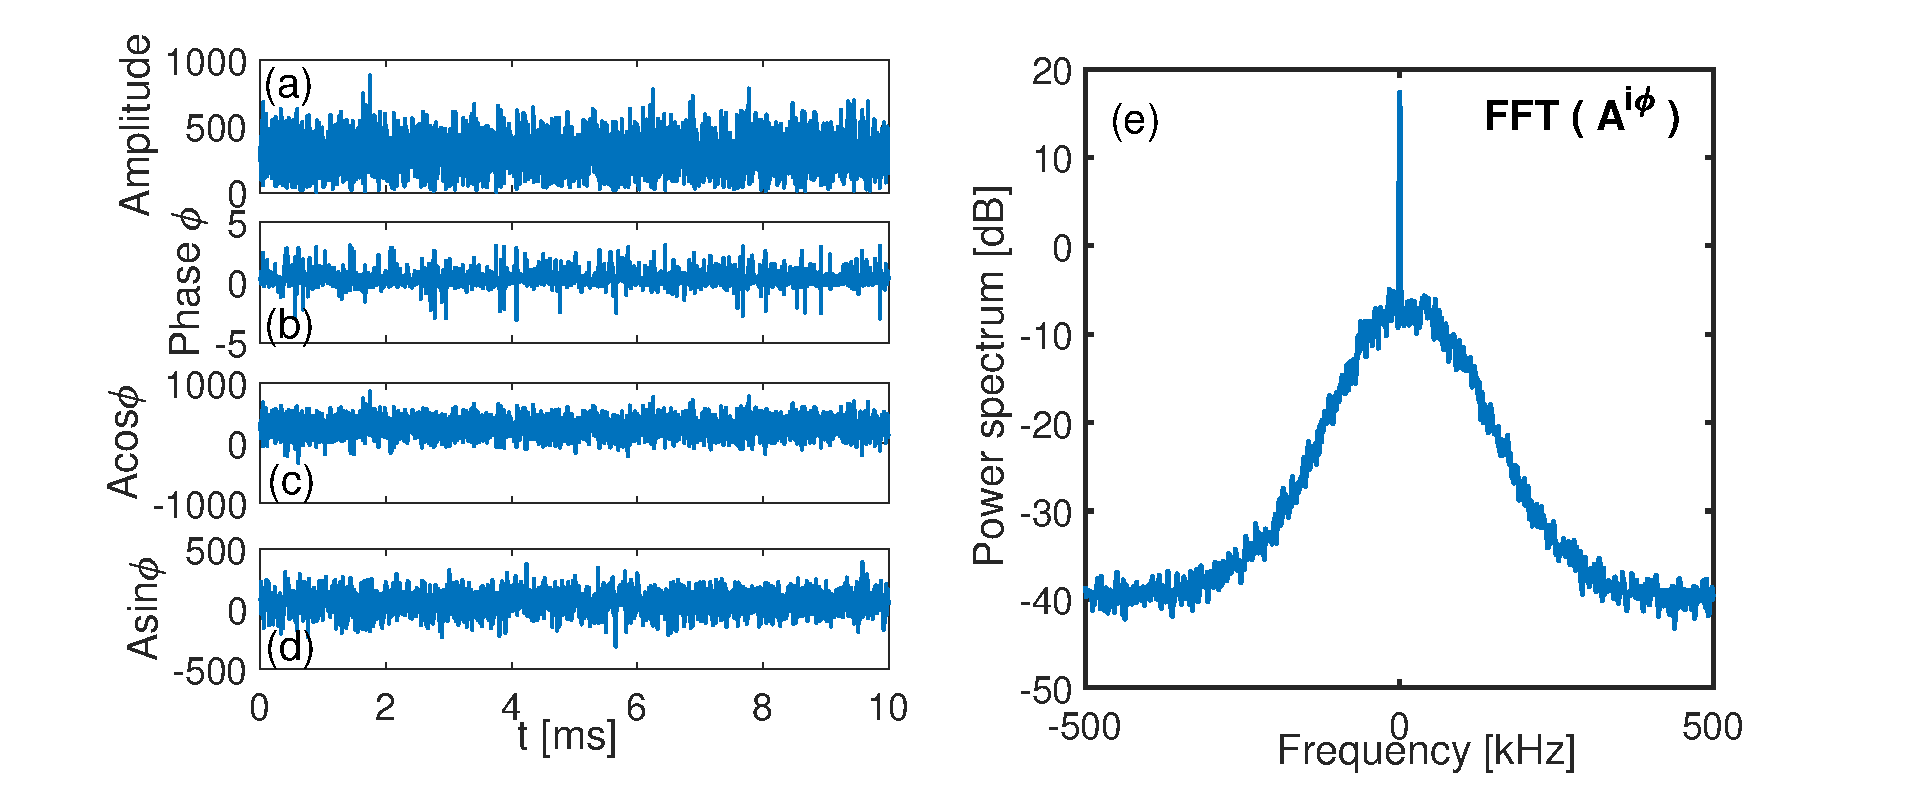
\includegraphics[scale=0.45]{signal.eps}
\par\end{centering}
\caption[Fluctuation signals]{Raw fluctuation signals of (a) amplitude, (b) phase, (c) $Acos\phi$ and (d) $Asin\phi$ and (e) the corresponding power from the complex signal by the FFT algorithm, where the Welch method was used with Hamming window width 1024 and an overlap of 50\%.}
\label{fig:signal}
\end{figure}
%%%%%%%%%%%%%%%%%%%%


%%%%%%%%%%%%%%%%%%%%
\begin{figure}[!h]
\begin{centering}
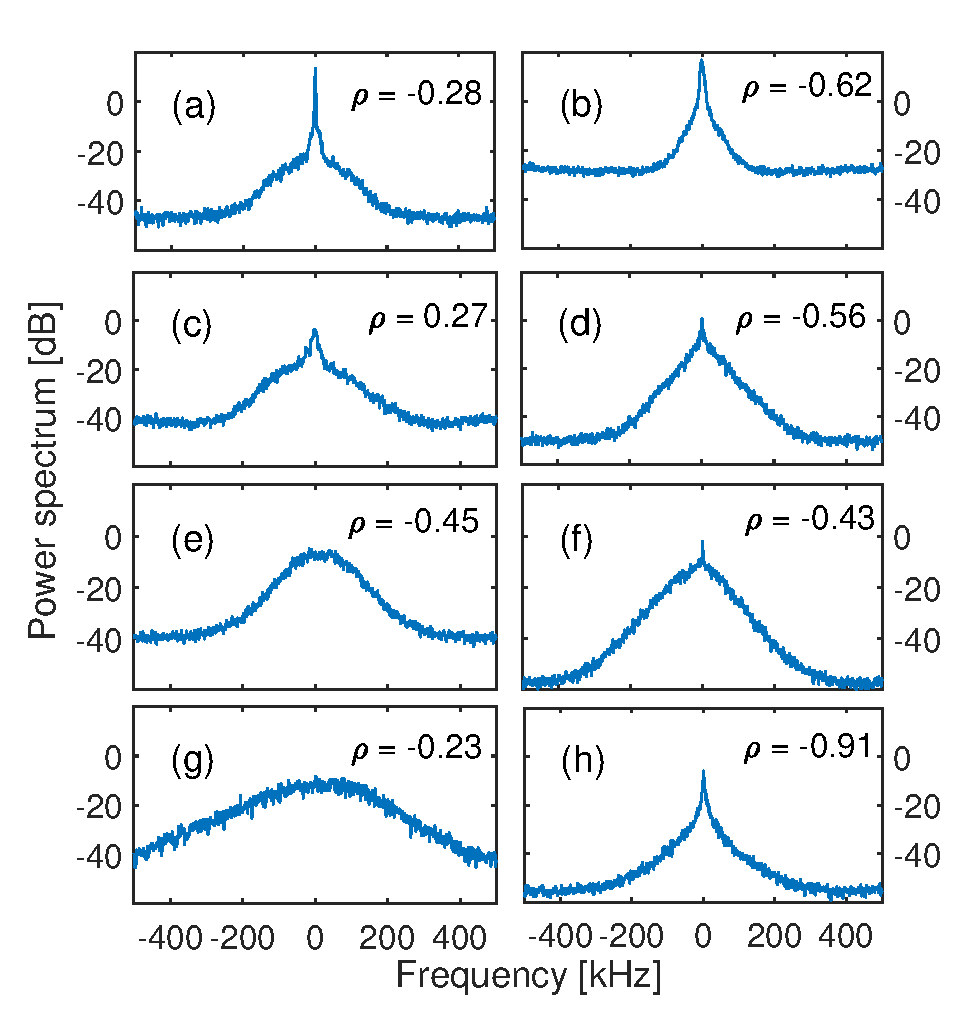
\includegraphics[scale=0.55]{fig_Spectra.eps}
\par\end{centering}
\caption[Representative spectra in the database]{Some typical frequency spectra obtained from the core reflectometer database, with 1024 frequency bins. The normalized radial position ($\rho$) of the cutoff layer was calculated from a density profile obtained by the interferometry diagnostic. Negative $\rho$ indicates HFS radial position.}
\label{fig:Spectra}
\end{figure}
%%%%%%%%%%%%%%%%%%%%



Furthermore, figure \ref{fig:Spectra} shows several other typical frequency spectra obtained from fluctuation measurements using this reflectometry setup, under different conditions and at varying radial positions. The spectra $S(f)$ ($f$ is frequency) are plotted on a logarithmic scale ($10 \times log_{10}(S)$ in units of decibel (dB)). Although not all possible shapes of the complicated and varying frequency spectra in Tore Supra plasmas are shown, the examples in figure \ref{fig:Spectra} do represent the typical spectral shape features encountered throughout the database. Positive and negative frequencies correspond to different directions of turbulence structure, respectively. The spectrum can be almost symmetrical, but sometimes the asymmetry is strong. This can be due to various reasons, like Doppler shift, small displacements of the plasma with respect to the equatorial plane, or asymmetries of the turbulent structures or in the wave propagation. As shown in figure \ref{fig:Spectra}, the fluctuation frequency spectra can be Gaussian-like (spectra (e) and (g)) or much more Lorentzian-like (spectrum (h)), i.e. strongly peaked with heavy tails. Other spectrum shapes are in between these typical spectra. The low-frequency component can be intense (spectra (a) and (b)), invisible (spectra (e) and (g)), or mixed with other parts of the spectrum (spectra (d) and (h)).


From reflectometry fluctuation power spectra, each spectrum has 1024 frequencies or parameters which is too much for a systematic study. Therefore, we follow a parametric approach to characterize the spectra by means of only a few parameters, i.e. a reduction from $10^3$ to ca. 10 parameters. This is the basic motivation for the parametrization method discussed in the next chapter.


